\documentclass[11pt,letterpaper,reqno]{article}

\textwidth      =  6in
\textheight     =  8.25in
\oddsidemargin  =  18pt
\evensidemargin =  18pt
\topmargin      =  0.00in

\usepackage[utf8]{inputenc}
\usepackage[spanish]{babel}
\usepackage{amsmath}
\usepackage{amsfonts}
\usepackage{amssymb}
\usepackage{graphicx}
\usepackage{minted}
\graphicspath{{img/}}

\title{Implementación y Simulaciones del Modelo $k$-nn}
\author{Abraham Toriz\\ Jesús Mejía\\ Luis Cortés\\ Roberto Saucedo}

\begin{document}
\maketitle
\begin{abstract}
En este trabajo se da la implementación  de del modelo $k$-nn, después se hacen simulaciones y se comentarios de los resultados obtenidos.
\end{abstract}

\section{Implementación en Python}
Sea \verb|data = |$\{(X_i, Y_i): i=1,\;2,\ldots,\;N,\; Y_i=1 \text{ ó } Y_i=2\}$ el conjunto de $N$ observaciones y \verb|x| un dato que queremos clasificar. En estos ejemplos, usaremos la métrica eucliana y los cálculos los hará la función \verb|metric(x, y)|.\\

Primero debemos calcular las todas distancias entre \verb|x| y los $X_i$ en \verb|data|
\begin{minted}{python}
    distances = []
    for dat in data:
        distances.append((metric(dat[0], x), dat[1]))
\end{minted}

Una vez guardadas las distancias, se ordenan ascendentemente, es decir:
\begin{minted}{python}
    distances.sort(key=lambda x: x[0])
\end{minted}
Luego se encuentra el número de elementos de la clase uno y de la clase dos para los $k$ vecinos más cercanos:
\begin{minted}{python}
    classes = {}
    for item in distances[:k]:
        if item[1] in classes:
            classes[item[1]] += 1
        else:
            classes[item[1]] = 1
\end{minted}
Finalmente se selecciona la clase con mayor número de elementos:
\begin{minted}{python}
    classes = list(classes.items())
    classes.sort(key=lambda x: x[1])
    return classes[-1][0]
\end{minted}

A continuación se da la función principal de este algoritmo.
\begin{minted}{python}
def k_nearest(data, x, metric=euclidean, k=11):

    distances = []
    for dat in data:
        distances.append((metric(dat[0], x), dat[1]))

    distances.sort(key=lambda x: x[0])

    # lets see which is the most common
    classes = {}
    for item in distances[:k]:
        if item[1] in classes:
            classes[item[1]] += 1
        else:
            classes[item[1]] = 1

    classes = list(classes.items())

    classes.sort(key=lambda x: x[1])

    return classes[-1][0]
\end{minted}

\section{Simulaciones}

A continuación se dan los resultados, las gráficas y el tiempo de ejecución de las simulaciones. Se considerarán la distribución Gaussiana con diferentes medias y varianzas. En todos los casos se considera $k=11$. Es preciso hacer notar que se clasificaron los los datos que están identificados con el color rojo.

\begin{figure}[h]
	\centering
	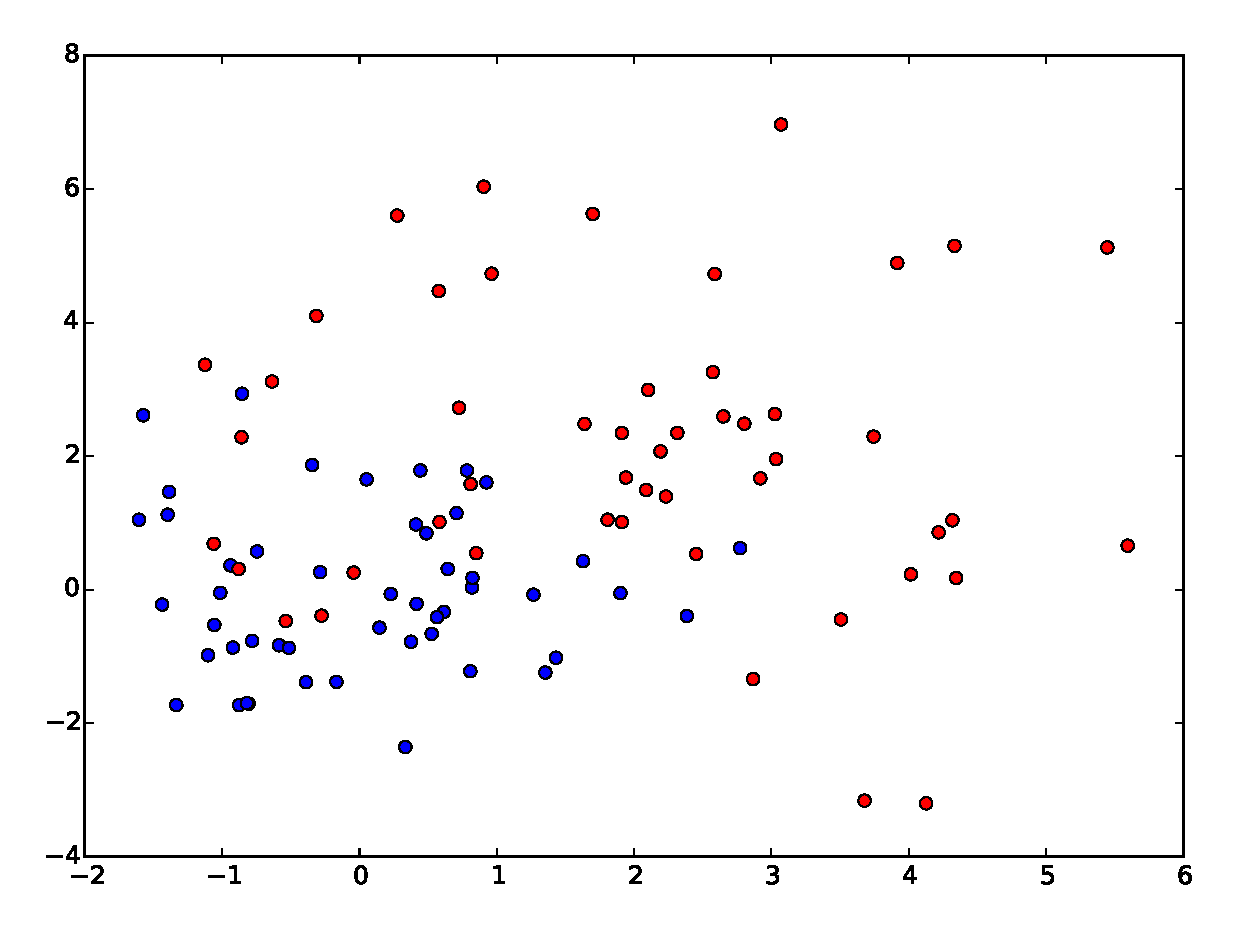
\includegraphics[scale=.5]{img1}
	\caption{Para 50 observaciones de dos Gaussinas con media 0.0 y 2.0, varianza 1.0 y 2.0, respectivamente. Se obtuvo el 82.0\% de aciertos. La ejecución duró 0.898 segundos.}
\end{figure}

\begin{figure}[h]
	\centering
	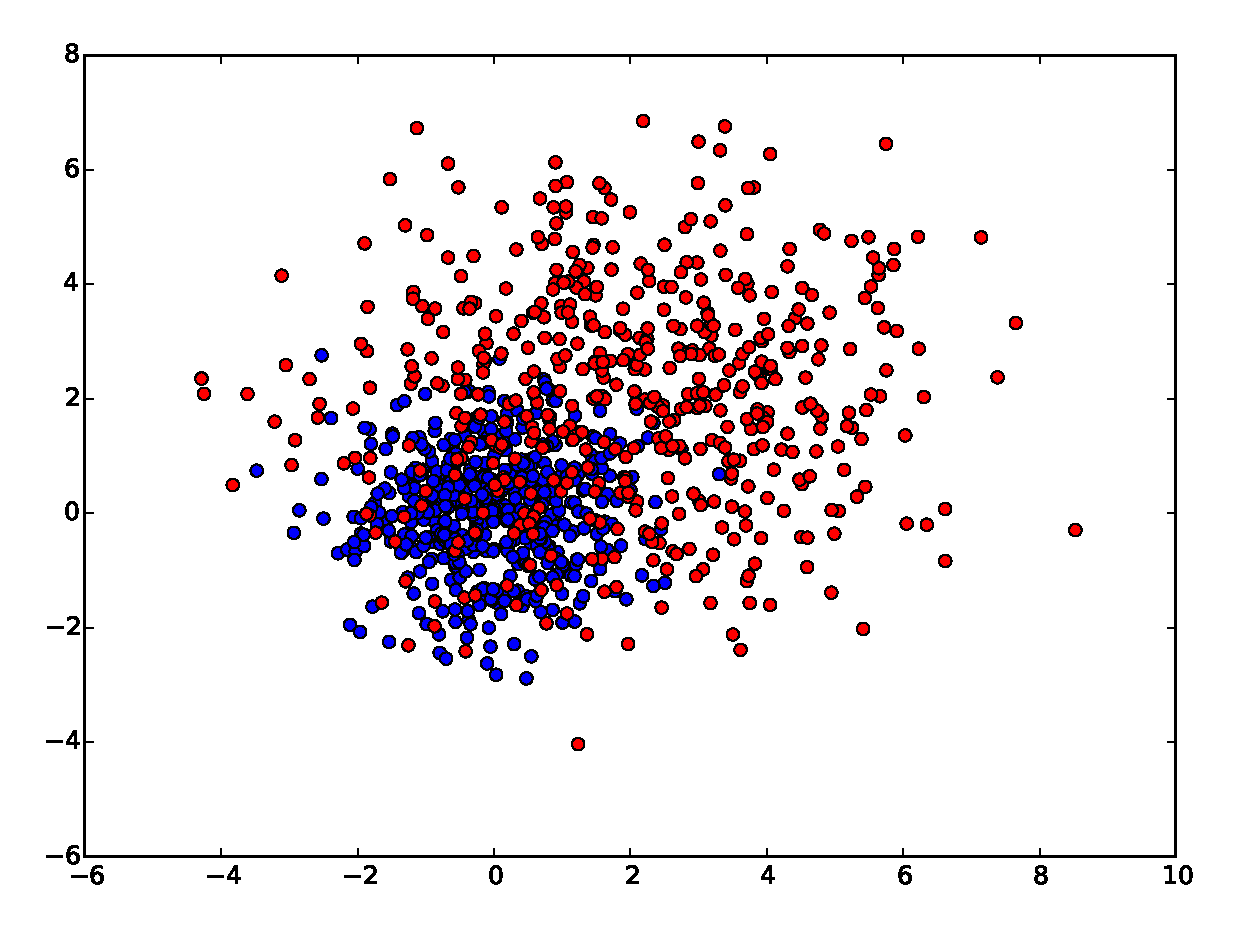
\includegraphics[scale=.5]{img2}
	\caption{Para 500 observaciones de dos Gaussinas con media 0.0 y 2.0, varianza 1.0 y 2.0, respectivamente. Se obtuvo el 81.0\% de aciertos. La ejecución duró 2.456 segundos.}
\end{figure}

\begin{figure}[h]
	\centering
	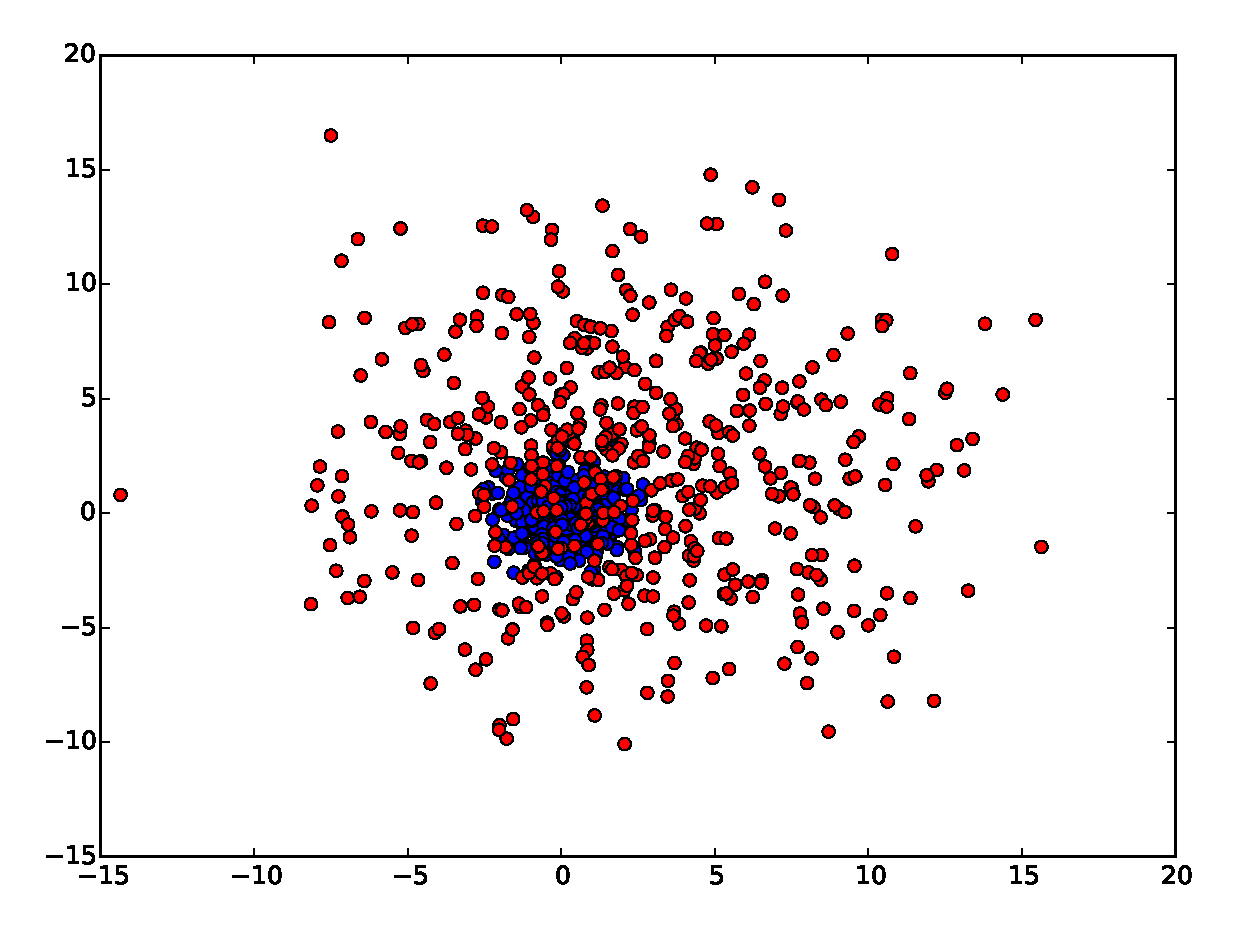
\includegraphics[scale=.5]{img3}
	\caption{Para 500 observaciones de dos Gaussinas con media 0.0 y 2.0, varianza 1.0 y 5.0, respectivamente. Se obtuvo el 89.4\% de aciertos. La ejecución duró 2.440. segundos.}
\end{figure}

\begin{figure}[h]
	\centering
	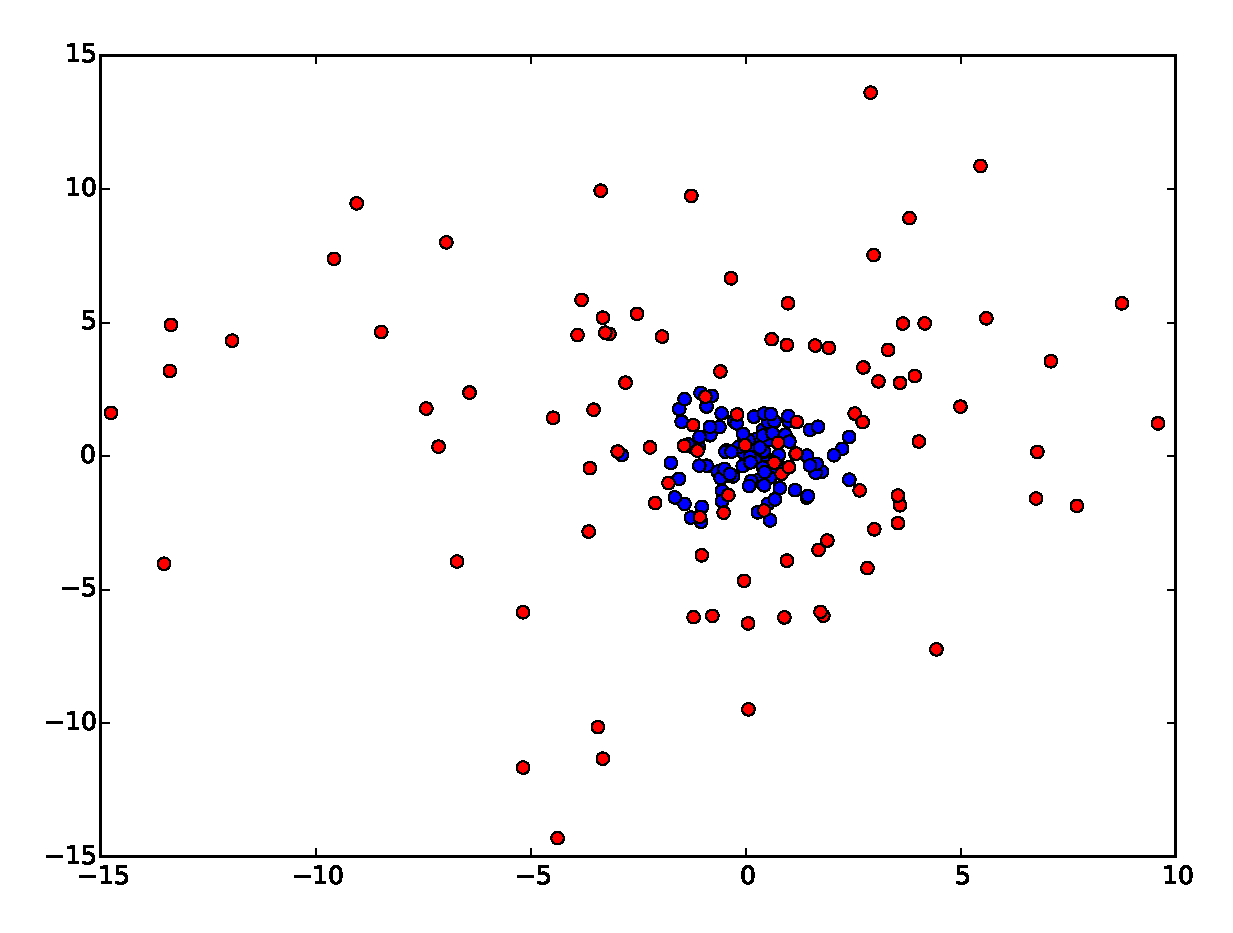
\includegraphics[scale=.5]{img4}
	\caption{Para 100 observaciones de dos Gaussinas con media 0.0 y 0.0, varianza 1.0 y 5.0, respectivamente. Se obtuvo el 82.0\% de aciertos. La ejecución duró 0.946 segundos.}
\end{figure}

\begin{figure}[h]
	\centering
	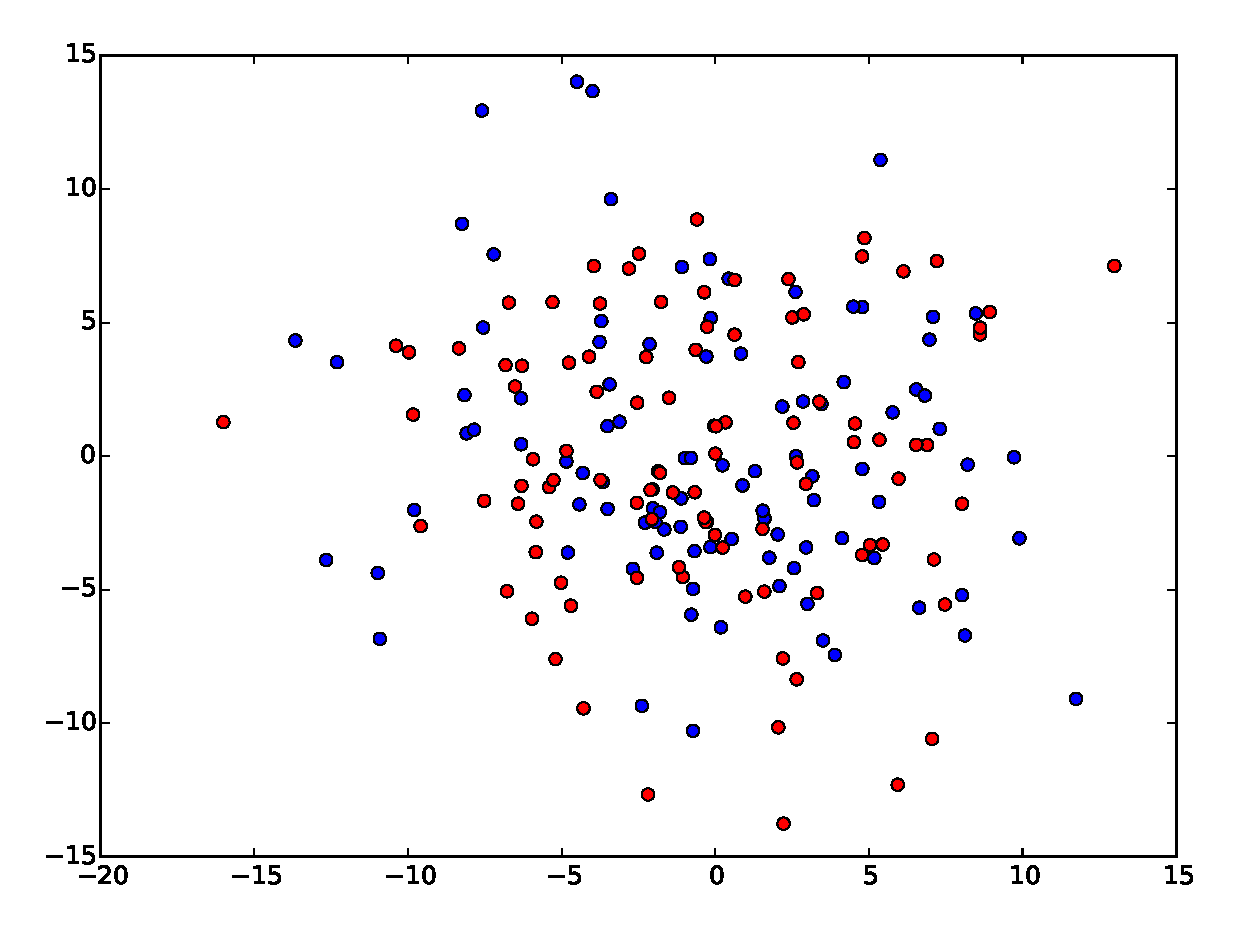
\includegraphics[scale=.5]{img5}
	\caption{Para 100 observaciones de dos Gaussinas con media 0.0 y 0.0, varianza 5.0 y 5.0, respectivamente. Se obtuvo el 57.0\% de aciertos. La ejecución duró 0.948 segundos.}
\end{figure}

\begin{figure}[h]
	\centering
	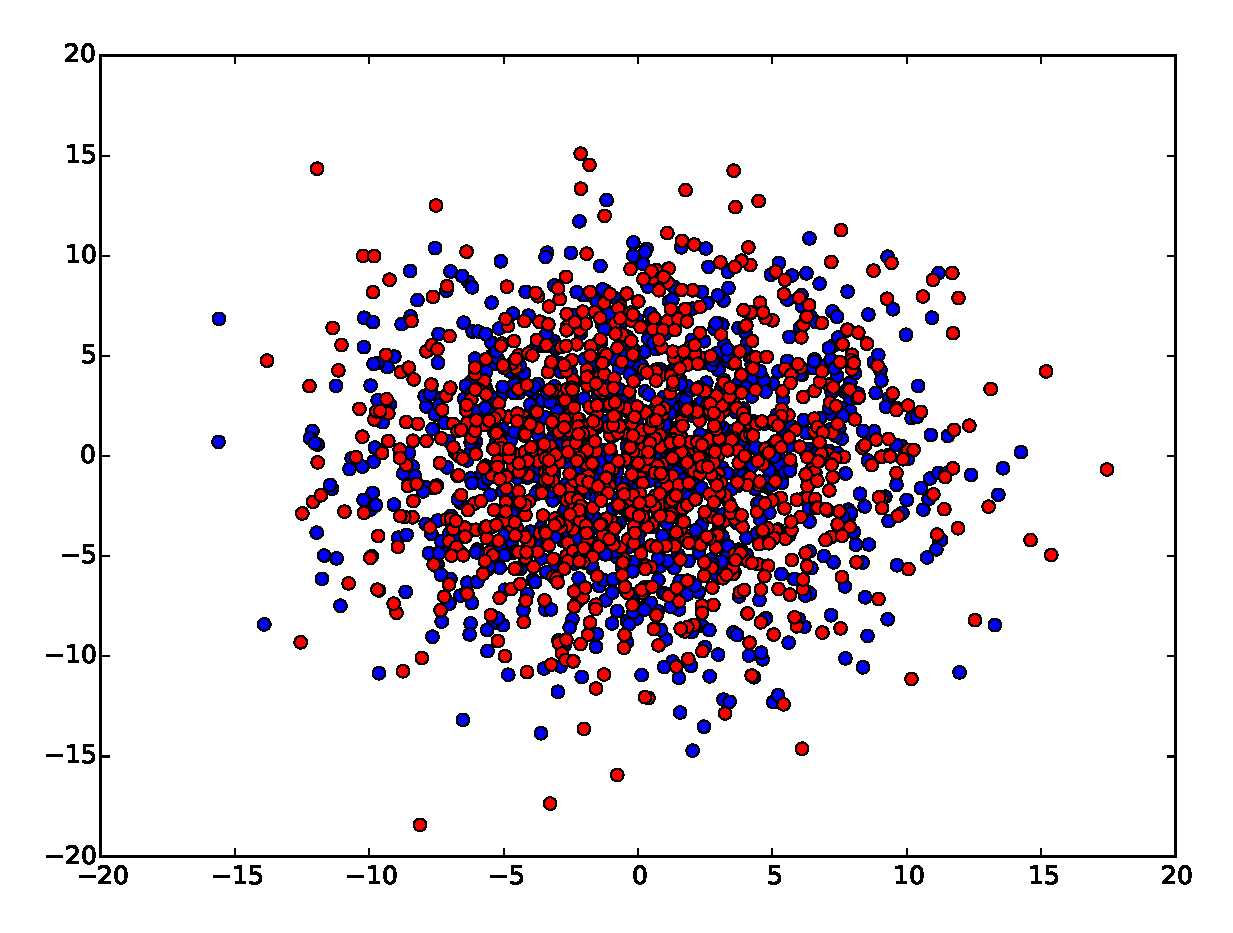
\includegraphics[scale=.5]{img6}
	\caption{Para 1000 observaciones de dos Gaussinas con media 0.0 y 0.0, varianza 5.0 y 5.0, respectivamente. Se obtuvo el 61.8\% de aciertos. La ejecución duró 7.237 segundos.}
\end{figure}

\begin{figure}[h]
	\centering
	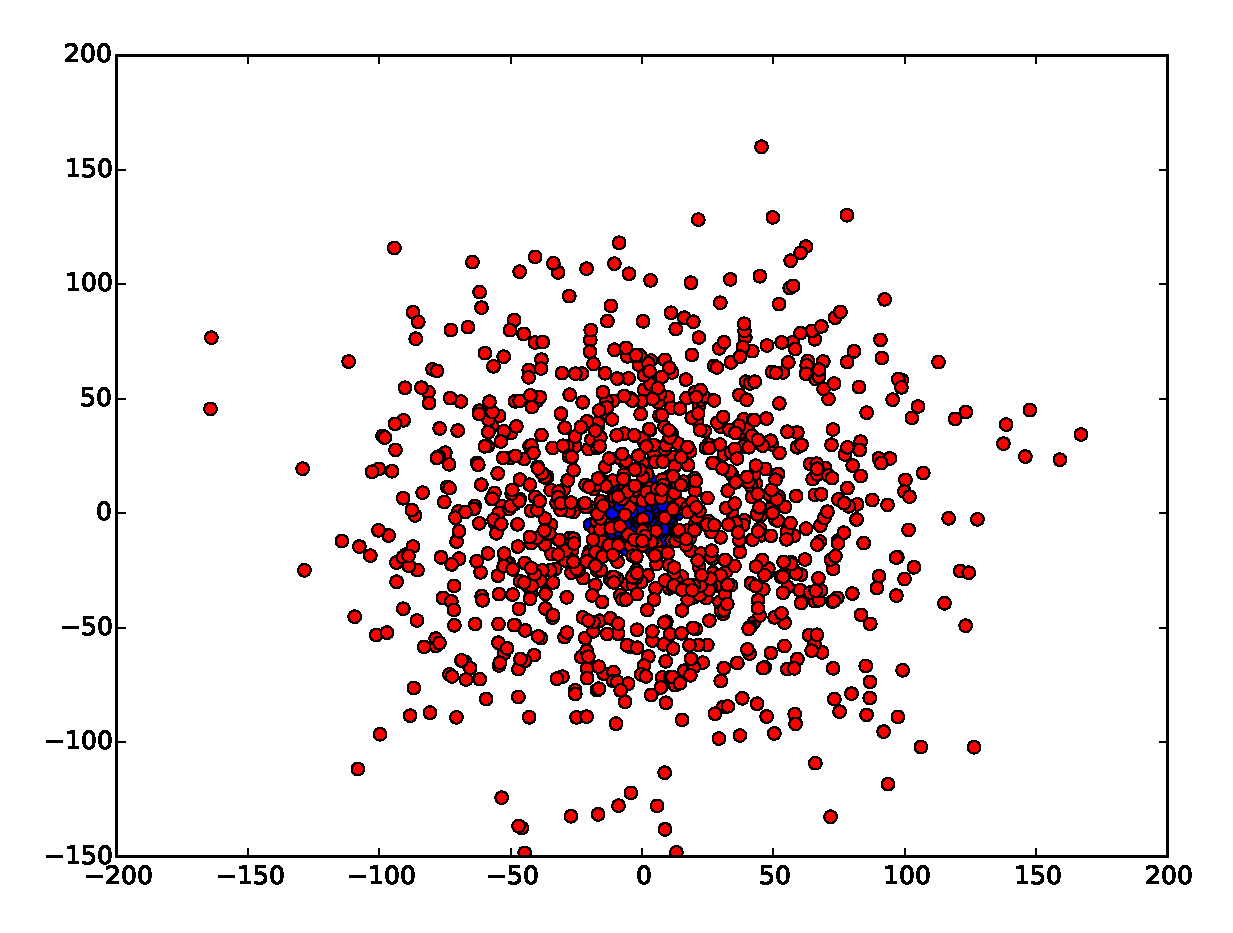
\includegraphics[scale=.5]{img7}
	\caption{Para 1000 observaciones de dos Gaussinas con media 0.0 y 0.0, varianza 5.0 y 50.0, respectivamente. Se obtuvo el 96.5\% de aciertos. La ejecución duró 7.204 segundos.}
\end{figure}

\begin{figure}[h]
	\centering
	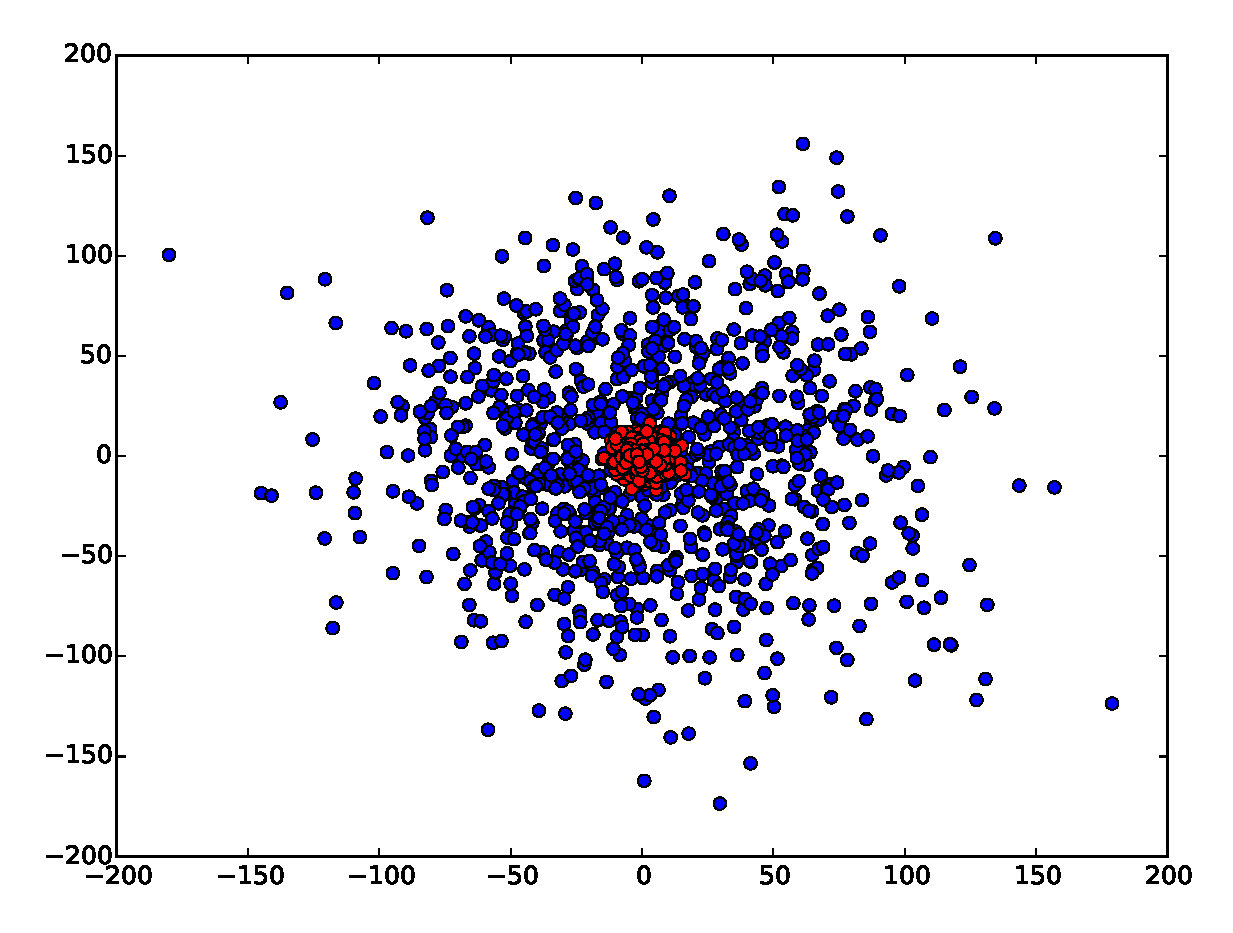
\includegraphics[scale=.5]{img8}
	\caption{Para 1000 observaciones de dos Gaussinas con media 0.0 y 0.0, varianza 50.0 y 5.0, respectivamente. Se obtuvo el 99.8\% de aciertos (en los elementos de color azul). La ejecución duró 7.200 segundos.}
\end{figure}

\begin{figure}[h]
	\centering
	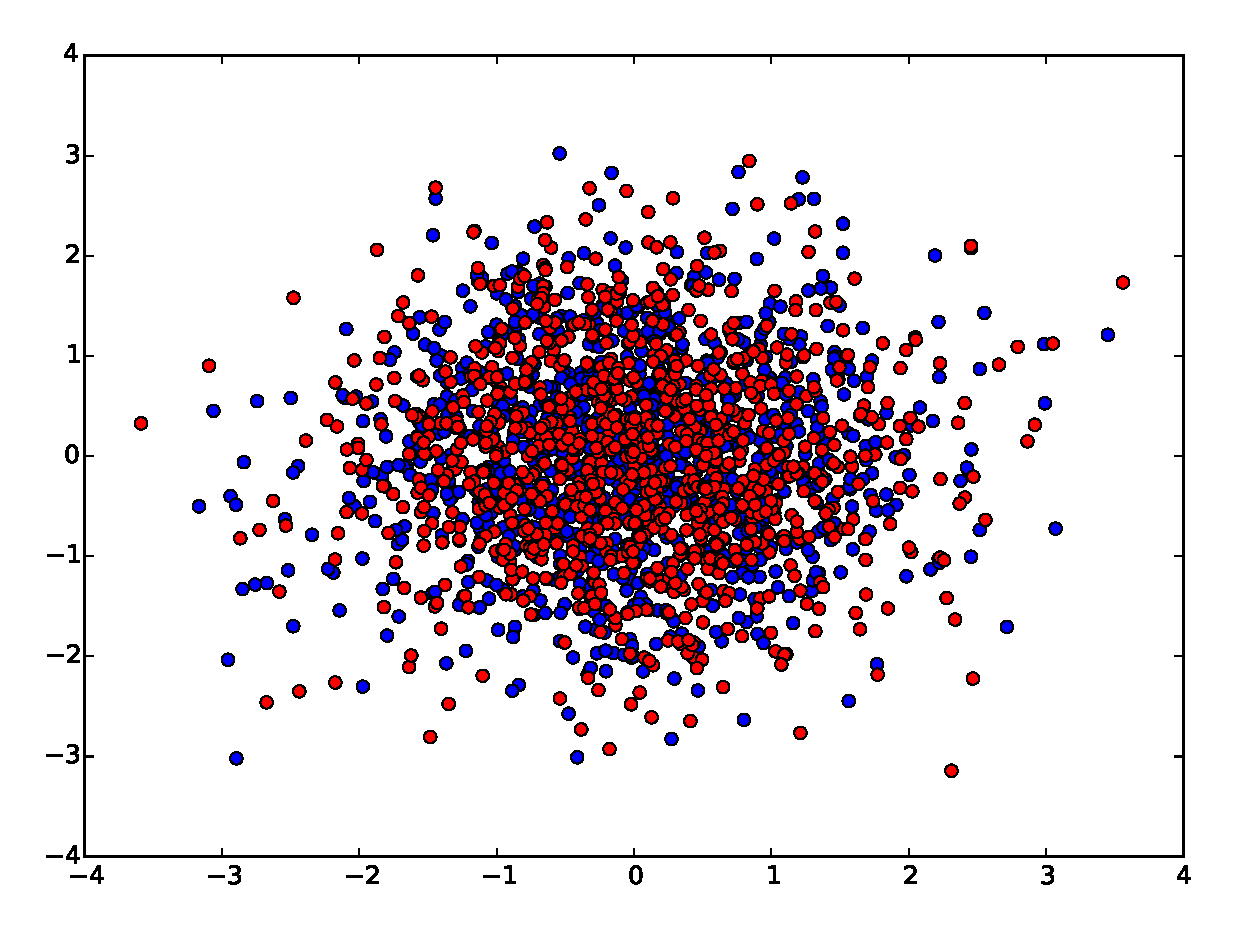
\includegraphics[scale=.5]{img9}
	\caption{Para 1000 observaciones de dos Gaussinas con media 0.0 y 0.0, varianza 1.0 y 1.0, respectivamente. Se obtuvo el 60.5\% de aciertos. La ejecución duró 7.379 segundos}
\end{figure}
\clearpage
\section{Conclusiones}
Notemos que este algoritmos es eficiente en la mayoría de los casos. Sin embargo, cuando la varianza de las distribuciones difiere muchos, entonces el algoritmos es poco factible. Por otro lado, notemos que el tiempo de ejecución es relativamente poco, a pesar de que el tamaño de la muestra, en algunos casos, rebasa los 500 datos de prueba.\\

En conclusión, si se requiere una clasificación rápida se recomienda este algoritmo, ya que su implementación no es muy complicada y se puede realizar en cualquier lenguaje de programación.
\end{document}